\hypertarget{dman3_8h}{
\subsection{dman3.h File Reference}
\label{dman3_8h}\index{dman3.h@{dman3.h}}
}


\subsubsection{Detailed Description}
DMAN3 Interface Definitions (C64P) - 3rd Generation DMAN. Application interface to the DMA Manager. Grants DMA resources to XDAIS algorithms. 



Definition in file \hyperlink{dman3_8h-source}{dman3.h}.

{\tt \#include $<$ti/xdais/ialg.h$>$}\par
{\tt \#include $<$ti/xdais/idma3.h$>$}\par


Include dependency graph for dman3.h:\begin{figure}[H]
\begin{center}
\leavevmode
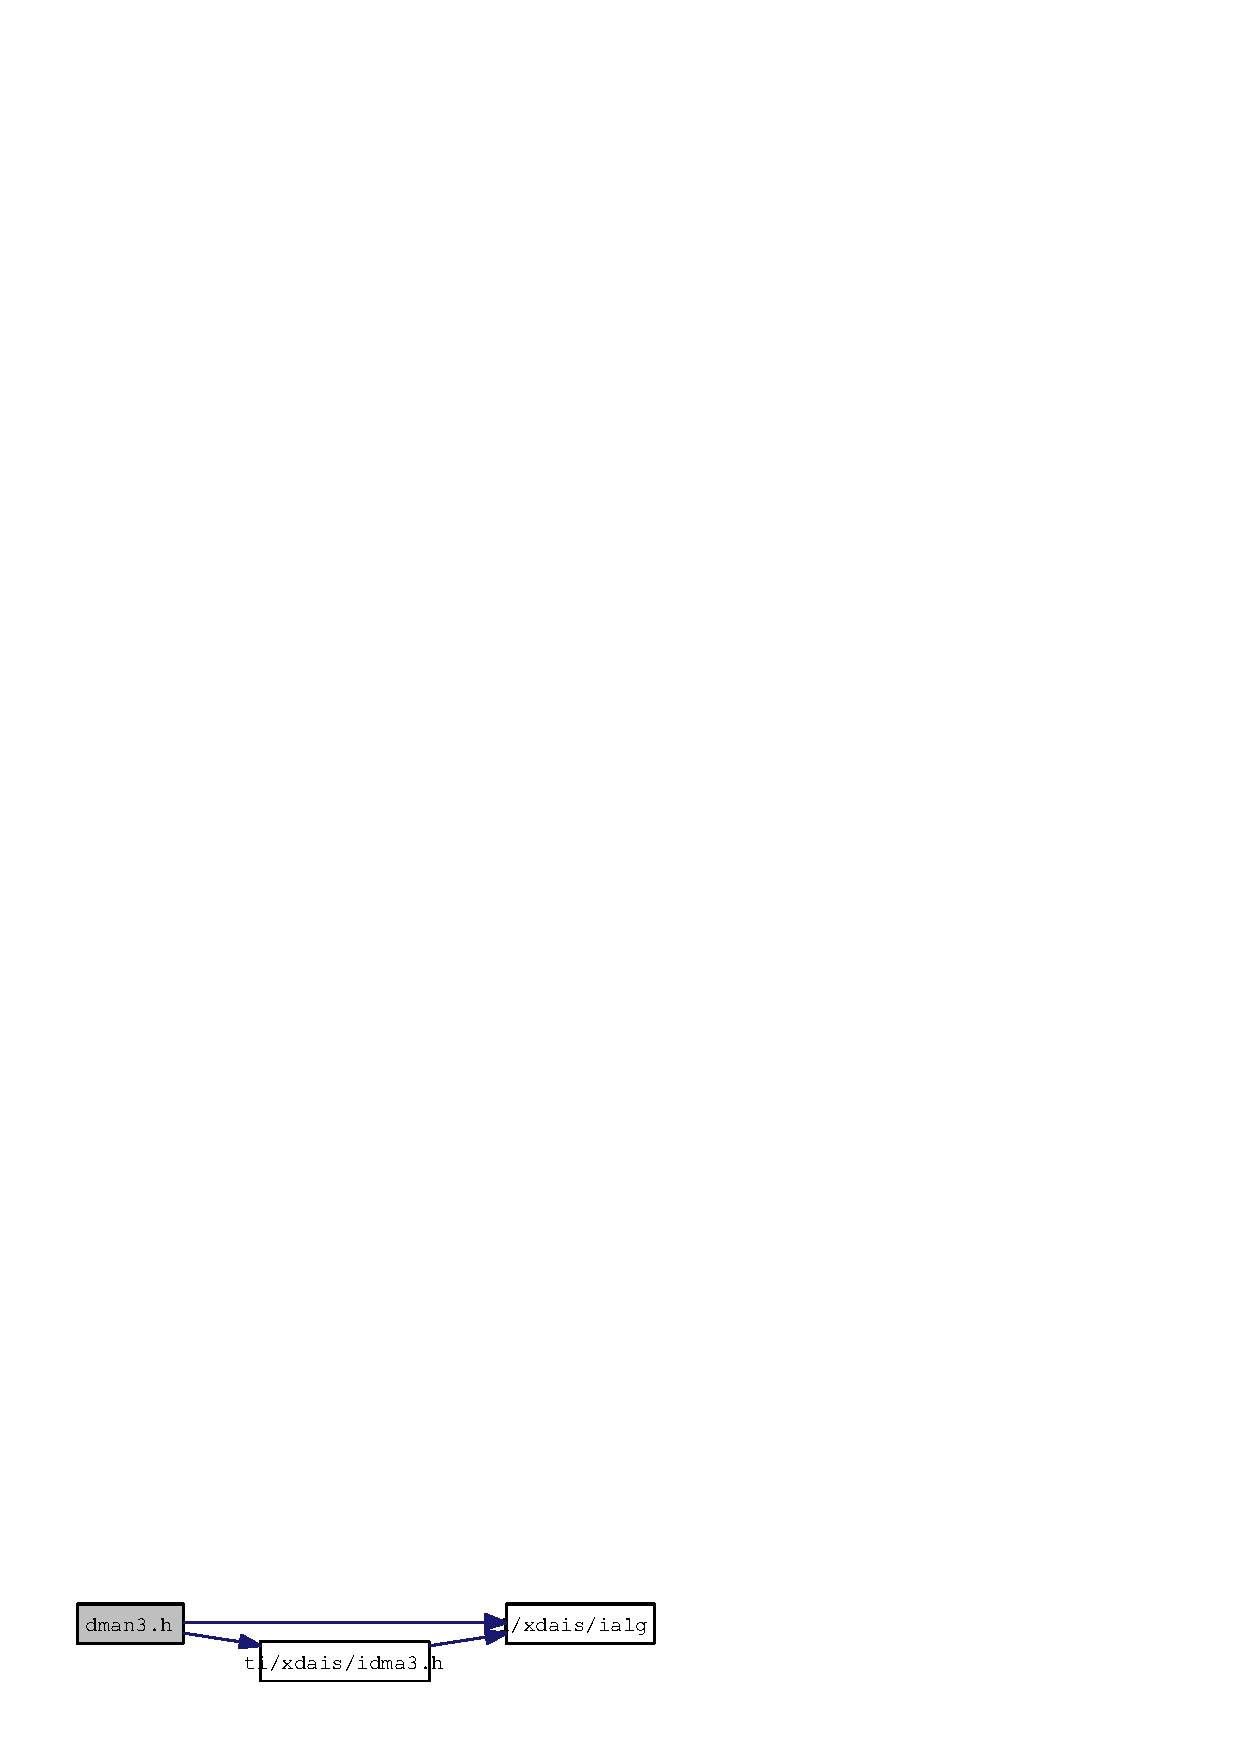
\includegraphics[width=157pt]{dman3_8h__incl}
\end{center}
\end{figure}
\subsubsection*{Data Structures}
\begin{CompactItemize}
\item 
struct \hyperlink{struct_d_m_a_n3___params}{DMAN3\_\-Params}
\begin{CompactList}\small\item\em The module configuration structure for DMAN3 implementation. It is set at design time by the system integrator to ensure optimal sharing of DMA resources for the execution environment. \item\end{CompactList}\end{CompactItemize}
\subsubsection*{Defines}
\begin{CompactItemize}
\item 
\#define \hyperlink{group___d_s_p_d_m_a_n3_gc5bb90e4340386e641863309330e4fb5}{DMAN3\_\-MAXDMARECS}~32
\item 
\#define \hyperlink{group___d_s_p_d_m_a_n3_gb4a261c271c8d0f1e9843eada6b263e8}{DMAN3\_\-MAXGROUPS}~20
\end{CompactItemize}
\begin{Indent}{\bf Defines: DMAN3 Status Codes}\par
\begin{CompactItemize}
\item 
\#define \hyperlink{group___d_s_p_d_m_a_n3_g462d3887266b42b69cf21c65e87dc99d}{DMAN3\_\-SOK}~0
\item 
\#define \hyperlink{group___d_s_p_d_m_a_n3_g70d091dae946805ff49ab47b903483a7}{DMAN3\_\-EOUTOFMEMORY}~-1
\item 
\#define \hyperlink{group___d_s_p_d_m_a_n3_ge81e9235f9755ac2e6a6279401c8798d}{DMAN3\_\-EFAIL}~-2
\item 
\#define \hyperlink{group___d_s_p_d_m_a_n3_g097f382f6603cc69c2d998c0ce6b9dfe}{DMAN3\_\-EFREE}~-3
\item 
\#define \hyperlink{group___d_s_p_d_m_a_n3_gb04511fe9f738b3a189758163e75f1d2}{DMAN3\_\-EOUTOFTCCS}~-4
\item 
\#define \hyperlink{group___d_s_p_d_m_a_n3_g45977d32b34b6e98e33b6510c9164dee}{DMAN3\_\-EOUTOFPARAMS}~-5
\end{CompactItemize}
\end{Indent}
\subsubsection*{Typedefs}
\begin{CompactItemize}
\item 
typedef Bool($\ast$) \hyperlink{group___d_s_p_d_m_a_n3_gb88a4f4fc347844728e7c0d6b46c5ecf}{DMAN3\_\-Scratch\-Alloc\-Fxn} (\hyperlink{struct_i_a_l_g___obj}{IALG\_\-Handle} alg, Int mutex\-Id, \hyperlink{struct_i_a_l_g___mem_rec}{IALG\_\-Mem\-Rec} $\ast$mem\-Tab, Int num\-Recs)
\begin{CompactList}\small\item\em Function prototype for allocating IDMA3 Object's env from shared scratch memory. Algorithms might specify a particular IDMA3 protocol that provides custom DMA services. This protocol might require extra memory for the IDMA3 object's environment. DMAN3\_\-Scratch\-Alloc\-Fxn might be used to allocate this memory. If this is NULL, then the env will be allocated from persistent memory. \item\end{CompactList}\item 
typedef Void($\ast$) \hyperlink{group___d_s_p_d_m_a_n3_g5c51dee2c06d775005a8cf4db004782f}{DMAN3\_\-Scratch\-Free\-Fxn} (Int mutex\-Id, Void $\ast$addr, Uns size)
\begin{CompactList}\small\item\em Function prototype for freeing IDMA3 Object's env from shared scratch memory. If this is NULL then env will be freed from persistent memory. \item\end{CompactList}\end{CompactItemize}
\subsubsection*{Functions}
\begin{CompactItemize}
\item 
Int \hyperlink{group___d_s_p_d_m_a_n3_ge0e5031bc5e947da1bd5d12cca1c5e00}{DMAN3\_\-grant\-Dma\-Channels} (Int group\-Id, \hyperlink{struct_i_a_l_g___obj}{IALG\_\-Handle} alg\-Handle\mbox{[}$\,$\mbox{]}, \hyperlink{struct_i_d_m_a3___fxns}{IDMA3\_\-Fxns} $\ast$dma\-Fxns\mbox{[}$\,$\mbox{]}, Int num\-Algs)
\begin{CompactList}\small\item\em Add one or several algorithms to the DMA Manager. The DMA Manager will grant DMA resources to the algorithms as a result. This function is called when initializing XDAIS algorithm instances. \item\end{CompactList}\item 
Void \hyperlink{group___d_s_p_d_m_a_n3_gc26a2a6153c50b10dc3ae9106bfa8594}{DMAN3\_\-exit} (Void)
\begin{CompactList}\small\item\em Finalization method of the DMAN module. \item\end{CompactList}\item 
Int \hyperlink{group___d_s_p_d_m_a_n3_gee927c5ad460e5e5a122471ccb047db1}{DMAN3\_\-create\-Channels} (Int group\-Id, \hyperlink{struct_i_d_m_a3___channel_rec}{IDMA3\_\-Channel\-Rec} dma\-Tab\mbox{[}$\,$\mbox{]}, Int num\-Chans)
\begin{CompactList}\small\item\em Allocate and initialize memory for one or several channel handles. \item\end{CompactList}\item 
Void \hyperlink{group___d_s_p_d_m_a_n3_gf0a672c8ba5962dabc8b319978aafd3b}{DMAN3\_\-init} (Void)
\begin{CompactList}\small\item\em Initialization method of the DMAN3 module. \hyperlink{group___d_s_p_d_m_a_n3_gf0a672c8ba5962dabc8b319978aafd3b}{DMAN3\_\-init()} uses externally configured and provided DMAN3\_\-PARAMS to initialize DMAN3 resources (QDMA channel map, memory heap...). \item\end{CompactList}\item 
Int \hyperlink{group___d_s_p_d_m_a_n3_g664b5e2445c2ec3a0ed9e14f8cfc1d20}{DMAN3\_\-release\-Dma\-Channels} (\hyperlink{struct_i_a_l_g___obj}{IALG\_\-Handle} alg\-Handle\mbox{[}$\,$\mbox{]}, \hyperlink{struct_i_d_m_a3___fxns}{IDMA3\_\-Fxns} $\ast$dma\-Fxns\mbox{[}$\,$\mbox{]}, Int num\-Algs)
\begin{CompactList}\small\item\em Remove logical channel resources from one or several algorithm instances. \item\end{CompactList}\item 
Int \hyperlink{group___d_s_p_d_m_a_n3_g2d14c4952c1194b913ac6e8bb7f0e9d5}{DMAN3\_\-free\-Channels} (\hyperlink{struct_i_d_m_a3___obj}{IDMA3\_\-Handle} channel\-Tab\mbox{[}$\,$\mbox{]}, Int num\-Chans)
\begin{CompactList}\small\item\em Free memory for array of channel handles. \item\end{CompactList}\end{CompactItemize}
\subsubsection*{Variables}
\begin{CompactItemize}
\item 
far \hyperlink{struct_d_m_a_n3___params}{DMAN3\_\-Params} \hyperlink{group___d_s_p_d_m_a_n3_g553609efedb936222e4492f0ffa3d1cc}{DMAN3\_\-PARAMS}
\begin{CompactList}\small\item\em Default module configuration structure (defined in dman3.c). \item\end{CompactList}\end{CompactItemize}
